\chapter{HistoryFinder: Reliable Oracle Construction and Method-History Generation}
\label{ch:hf}

This chapter begins Part~\ref{part:test-method-evolution} and presents the second contribution of this thesis: improving the reliability of method-level history generation. Many software-evolution studies rely on accurate histories of individual methods, including studies of change-proneness, bug-proneness, technical debt, and test-code evolution. In this thesis, such histories are also required for Chapter~\ref{ch:t2p}, where we evaluate test-method history construction and then study test-method evolution. Therefore, this chapter addresses two related methodological problems: constructing reliable method-history oracles and improving tool support for method-history generation.

This chapter is based on the following manuscript:
\begin{itemize}
\item S. Islam, A. Aowal, M. S. Uddin, and S. Chowdhury, ``HistoryFinder: Advancing Method-Level Source Code History Generation with Accurate Oracles and Enhanced Algorithm,'' in Proceedings of the 48th IEEE/ACM International Conference on Software Engineering (ICSE 2026), Rio de Janeiro, Brazil, Apr. 2026.
\end{itemize}

The study revisits the evaluation of method-level history generation tools by constructing two systematically validated oracles: a corrected \textit{CodeShovel} oracle and a new \textit{HistoryFinder} oracle. Using these oracles, the study evaluates existing tools to identify their strengths and limitations before introducing \textit{HistoryFinder}. The evaluation uses 400 methods from 40 open-source Java repositories and compares \textit{HistoryFinder} with \textit{CodeShovel}, \textit{CodeTracker}, \textit{IntelliJ}, and \texttt{Git}-based baselines in terms of precision, recall, F1 score, and runtime.

The main takeaways from this chapter are as follows:
\begin{itemize}
\item Existing method-history oracles contain missing and incorrect method revisions, which can affect conclusions about tool performance.
\item Systematically validated oracles provide a more reliable basis for evaluating method-history generation tools.
\item Existing tools have different strengths and limitations when evaluated against more reliable oracles.
\item \textit{HistoryFinder} provides the strongest overall balance of precision, recall, F1 score, and runtime among the evaluated research tools.
\item The oracles and tool developed in this chapter support Chapter~\ref{ch:t2p}, where \textit{HistoryFinder} is evaluated on test-method history construction and then applied to method-level test-code evolution.
\end{itemize}

\textbf{Impact:} This work has been published in the Proceedings of the 48th IEEE/ACM International Conference on Software Engineering (ICSE 2026). Within this thesis, this chapter improves both benchmark quality and tool support for method-history generation. More broadly, its validated oracles and \textit{HistoryFinder} tool can support empirical studies that require accurate method histories, including studies of change-proneness, bug-proneness, technical debt, maintenance effort, code ownership, and software evolution. In this thesis, the contribution is further used in Chapter~\ref{ch:t2p} to study test-code evolution at the method level.



\section*{Abstract}
Reconstructing a method’s change history efficiently and accurately is critical for many software engineering tasks, including maintenance, refactoring, and comprehension. Despite the availability of method history generation tools such as \textit{CodeShovel} and \textit{CodeTracker}, existing evaluations of their effectiveness are limited by inaccuracies in the ground truth oracles used. In this study, we systematically construct two new oracles—the corrected \textit{CodeShovel} oracle and a newly developed \emph{HistoryFinder oracle}—by combining automated analysis with expert-guided manual validation. We also introduce \textit{HistoryFinder}, a new method history generation tool designed to improve not only the accuracy and completeness of method change histories but also to offer competitive runtime performance. Through extensive evaluation across 400 methods from 40 open-source repositories, we show that \textit{HistoryFinder} consistently outperforms \textit{CodeShovel}, \textit{CodeTracker}, \textit{IntelliJ}, and \texttt{Git-based} baselines in terms of precision, recall, and F1 score. Moreover, \textit{HistoryFinder} achieves competitive runtime performance, offering the lowest mean and median execution times among all the research-based tools. While \texttt{Git-based} tools exhibit the fastest runtimes, this efficiency comes at the cost of significantly lower precision and recall—leaving \textit{HistoryFinder} as the best overall choice when both accuracy and efficiency are important. To facilitate adoption, we provide a web interface, CLI, and Java library for flexible usage.

\section{Introduction}
Source code change history is valuable to both software practitioners and researchers. Practitioners leverage source code history for tasks such as code reviews, expert identification, and developer onboarding~\cite{grund_codeshovel_2021}. Researchers, on the other hand, use code history for a variety of tasks, including bug prediction~\cite{chowdhury_method-level_2024, mashhadi_empirical_2024}, code clone management~\cite{duala-ekoko_tracking_2007}, entity name recommendation~\cite{kashiwabara_method_2015}, security vulnerability detection \cite{li_cleanvul_2024}, code review \cite{grund_codeshovel_2021}, authorship attribution ~\cite{meng_mining_2013, rahman_ownership_2011}, and software maintenance effort estimation~\cite{chowdhury_good_2025, chowdhury_evidence_2025, hassan_versioned_2024}. To extract this historical information, researchers primarily relied on version control systems (VCS). However, traditional \texttt{VCSs} like \texttt{Git} mainly focus on file-level change tracking, which lacks the granularity needed for studies at finer levels. In practice, understanding maintenance activities at lower granularities—particularly at the method level—is important to both researchers and practitioners~\cite{grund_codeshovel_2021, chowdhury_evidence_2025, chowdhury_method-level_2024}. However, tracking method-level change history is challenging, as methods may be renamed or moved across files during refactoring and other development activities. These challenges and practical demands have driven the development of specialized tools for generating method-level change histories~\cite{higo_tracking_2020, grund_codeshovel_2021, jodavi_accurate_2022}.

Several approaches have been proposed to recover method-level code evolution, particularly from \texttt{Git} repositories. Hata \textit{et al.}~\cite{hata_historage_2011} introduced \textit{Historage}, a tool that enables method-level change tracking by restructuring repositories to store individual methods in separate files. This approach was later refined in \textit{FinerGit}~\cite{higo_tracking_2020}, which enhanced the accuracy of detecting small method changes. However, both tools require extensive preprocessing~\cite{grund_codeshovel_2021} of the codebase before any method-level history can be generated. This introduces additional storage overhead and preprocessing time, making them impractical for scenarios where fast and on-demand change history extraction is needed.

To mitigate the need for upfront preprocessing, Grund \textit{et al.} ~\cite{grund_codeshovel_2021} introduced \textit{CodeShovel} (ICSE 2021), a tool that tracks method-level change history on demand using a lightweight string similarity algorithm. \textit{CodeShovel} was reported to be both accurate and efficient, based on evaluation using a human-generated change history oracle of 200 Java methods. Unfortunately, Jodavi \textit{et al.}~\cite{jodavi_accurate_2022} later identified inaccuracies in this oracle. They corrected the oracle and introduced a more robust and refactoring-aware tool,  \textit{CodeTracker} (ESEC/FSE 2022), which significantly outperformed \textit{CodeShovel} in terms of precision and recall.

A concern remains, however, that the internal threats present in the human-generated \textit{CodeShovel} oracle may have carried over into the \textit{CodeTracker} oracle, which was largely derived from \textit{CodeShovel} and later corrected by a separate group of researchers, thereby introducing its own set of internal threats. Such inaccuracies in recorded change histories are particularly problematic, as tools validated by these oracles form the foundation for research on method-level maintenance analysis and modeling~\cite{ahmad_impact_2025, chowdhury_evidence_2025, chowdhury_good_2025, chowdhury_method-level_2024, chowdhury_revisiting_2022}. Moreover, the accuracy of tools evaluated against these less reliable oracles remains uncertain, raising concerns about their practical usefulness to software practitioners. Low precision in identifying method change commits can result in excessive false positives, while low recall may lead to missing critical changes—both of which can harm the usefulness of change history tracking in real-world scenarios.

To address the limitations of human-generated change histories, a more systematic, semi-automated approach was adopted to construct two new oracles for method-level change history. Rather than relying solely on manual annotation, A tool was developed to collect method-change commits for a given Java method using multiple state-of-the-art tools—namely, \textit{CodeShovel}, \textit{CodeTracker}, \textit{GitLog} (\textit{GitFuncName} and \textit{GitLineRange}), and \textit{IntelliJ}. The tool aggregates method change commits collected by all sources, based on the observation that this combined approach achieves significantly higher recall than any individual tool. This union set was then manually verified by two expert software engineers, who removed false positives to ensure high precision and added any relevant method change commits missed by all tools. The result is two high-quality oracles that combine the strengths of automated detection and expert validation. As shown later in the analysis (\textbf{RQ1}), the previously used oracles from \textit{CodeShovel} and \textit{CodeTracker} contain notable inaccuracies—confirming concerns about the validity of prior evaluations that relied on those oracles.

In addition to providing the new oracles, a novel, heuristic-based, method-level history generation algorithm and tool called \textit{HistoryFinder} is introduced. It also addresses several of \textit{CodeShovel}'s technical limitations. For instance, unlike \textit{CodeShovel}, \textit{HistoryFinder} captures changes introduced in merge commits, as well as modifications to JavaDocs, annotations, and code formatting.

\textit{HistoryFinder} is then compared with other method-level change-history tracking tools in terms of precision, recall, and runtime using the two newly developed oracles (\textbf{RQ2} and \textbf{RQ3}). Overall, the research-oriented tools—\textit{HistoryFinder}, \textit{CodeShovel}, and \textit{CodeTracker}—consistently demonstrate substantially higher accuracy than other alternatives such as \textit{GitLog} and \textit{IntelliJ}. \textit{HistoryFinder} generally achieves the highest precision and recall across all test oracles, while also offering competitive runtime performance. Although \textit{GitLog} is the fastest at reconstructing method histories, it suffers from significantly lower precision and recall, making \textit{HistoryFinder} the most balanced option in terms of accuracy and efficiency. To support broader adoption, a \texttt{GUI-based} tool is also provided that allows researchers and practitioners to generate method-level change histories using any of the state-of-the-art tools.

The contribution of this chapter can be summarized as follows.
\begin{itemize}
    \item It offers two systematically developed method-level change history oracles---consisting of 400 Java methods. Building these oracles with manual verification required approximately 300 hours from each of the two participating authors, excluding the time for building the necessary tools. These more accurate new oracles can be instrumental for future research on developing more method-level change history generation tools.
    \item It introduces a new algorithm and tool, \textit{HistoryFinder}, that addresses the limitations of the \textit{CodeShovel} tool.
    \item It conducts a thorough evaluation of the state-of-the-art method tracking tools against two accurate oracles to assess their relative performance in terms of precision, recall, F1 score, and runtime efficiency.
    \item It provides a user-friendly GUI-based tool that integrates all the state-of-the-art method-tracking tools (excluding \textit{IntelliJ}), allowing users to analyze and generate method histories for any arbitrary Java method from a \texttt{Git-based} project.
\end{itemize}

The two oracles and the GUI-based history generation tool are publicly shared.\footnote{\textit{HistoryFinder}: \url{https://github.com/SQMLab/HistoryFinder}} While this \texttt{GUI-based} tool can be used by both practitioners and researchers, the shared repository also shows how to use the new \textit{HistoryFinder} tool from the command line for enabling research in \emph{mining software repositories}.

\section{Background and Related Work}
This section discusses earlier research that leveraged code change history, especially at the method level, to analyze and build maintenance models. It then discusses research that focused on building history construction tools.
\subsection{Research on Code Change History and Maintenance}
Software maintenance models commonly target the prediction of changes and bugs, as components that undergo frequent modifications or are tied to bug fixes are often harmful~\cite{chowdhury_good_2025, arvanitou_method_2017, di_grazia_code_2023,opu2025llm}. Early identification of such components can substantially lower future maintenance effort and cost~\cite{gunes_koru_identifying_2007, abbas_software_2020, chowdhury_good_2025, chowdhury_empirical_2022}. Leveraging various code metrics, Koru \textit{et al.}~\cite{gunes_koru_identifying_2007} built tree-based models to forecast change-prone classes. In a similar vein, Romano and Pinzger~\cite{romano_using_2011} applied code metrics to predict change-prone \texttt{Java} interfaces. Khomh \textit{et al.}~\cite{khomh_exploratory_2009} demonstrated that certain types of code smells can also signal classes likely to change. Bug prediction models pursue a similar objective to \textit{change-proneness} prediction models: identifying code elements—such as classes or files—that are more likely to contain bugs in future versions~\cite{aleithan_explainable_2021, alsolai_predicting_2018, basili_validation_1996, gil_correlation_2017, zimmermann_predicting_2007, kamei_defect_2016}. These studies, however, primarily focused on the class or file level, which has been reported as less useful by both practitioners and researchers~\cite{grund_codeshovel_2021, pascarella_performance_2020, giger_method-level_2012, chowdhury_method-level_2024}. For example, finding bugs in a class or file can be difficult due to its large size. Consequently, method-level change and bug prediction models have gained traction in recent years.

Method-level bug prediction has been studied by Giger \textit{et al.}~\cite{giger_method-level_2012}, Mo \textit{et al.}~\cite{mo_exploratory_2022}, Ferenc \textit{et al.}~\cite{ferenc_automatically_2020}, Shippey \textit{et al.}~\cite{shippey_so_2016}, Hata \textit{et al.}~\cite{hata_bug_2012}, Menzies \textit{et al.}~\cite{menzies_data_2007}, Pascarella \textit{et al.}~\cite{pascarella_performance_2020}, and Chowdhury \textit{et al.}~\cite{chowdhury_method-level_2024}. These studies heavily relied on constructing method-level change histories—either to build labeled datasets or to derive change metrics used as input features for machine learning models. For instance, Mo \textit{et al.}~\cite{mo_exploratory_2022} employed metrics such as the number of added and deleted lines within a method to predict its bug-proneness, a strategy also adopted by Pascarella \textit{et al.}~\cite{pascarella_performance_2020}. Chowdhury \textit{et al.}~\cite{chowdhury_method-level_2024} used method-level change history to identify bug-fixing commits and label methods as buggy or non-buggy. The accuracy of the tools used to construct method-level change histories is therefore critical, as inaccuracies can lead to erroneous change metrics and incorrect bug labels.

\subsection{Research on History Construction}
Earlier studies on method-level tracking in \texttt{Git} used separate files to record method changes alongside \texttt{Git’s} file-level history. After extensive preprocessing of the entire codebase, this approach enables the use of \texttt{git log} to retrieve method histories. Hata \textit{et al.}~\cite{hata_historage_2011} introduced this technique with \textit{Historage}, which tracks changes to constructors, methods, and fields. However, Higo \textit{et al.}~\cite{higo_tracking_2020} found that \textit{Historage} struggles to track small methods when renamed or moved across files. To overcome these issues, they proposed \textit{FinerGit}, which represents methods with one token per line and applies heuristics for change comparison. Still, the preprocessing is time-intensive and incurs significant storage overhead—an issue common across similar tools~\cite{kim_when_2005,tu_integrated_2002,zimmermann_fine-grained_2006,hassan2004c}. Other tools~\cite{huang_cldiff_2018,falleri_fine-grained_2024} analyze changes between two versions but fall short of supporting origin analysis required by developers~\cite{grund_codeshovel_2021} and researchers~\cite{chowdhury_good_2025}.

Recent studies have proposed solutions that eliminate the need for upfront repository preprocessing and avoid tracking methods at each \texttt{Git} commit~\cite{jodavi_accurate_2022, grund_codeshovel_2021}. Grund \textit{et al.}~\cite{grund_codeshovel_2021} introduced \textit{CodeShovel}, a state-of-the-art tool capable of recovering method histories despite various transformations. On a manually annotated oracle, \textit{CodeShovel} outperformed both research tools (e.g., \textit{FinerGit}) and industry tools (e.g., \textit{IntelliJ}, \textit{GitLog}). However, Jodavi \textit{et al.}~\cite{jodavi_accurate_2022} found that \textit{CodeShovel} struggles when methods undergo significant body changes, such as during moves, often failing to track them correctly or misattributing their origin.

By leveraging the RefactoringMiner~\cite{tsantalis_refactoringminer_2022}, the authors also noted inaccuracies in the original \textit{CodeShovel} oracle and revised it based on their interpretation to create a more reliable benchmark. In general, they identified inaccuracies in 27 method histories due to method extraction refactorings. The authors updated the \textit{CodeShovel} oracle based on RefactoringMiner’s suggestions, but this approach has two key issues: (i) the accuracy of the remaining 173 methods is unknown, and (ii) RefactoringMiner itself has low recall (54.2) for the extract and move method~\cite{tsantalis_refactoringminer_2022}, raising doubts about the updates’ reliability. The authors also developed \textit{CodeTracker}, which employs RefactoringMiner’s advanced entity matching algorithm~\cite{tsantalis_refactoringminer_2022}. When evaluated with the new oracle, \textit{CodeTracker} showed significant improvements in precision and recall over \textit{CodeShovel}, but its reliance on RefactoringMiner introduced a performance bottleneck, making it significantly slower.

\emph{\textbf{Motivation:}} Like its predecessor, the new \textit{CodeTracker} oracle remains subject to internal validity threats, as it relies on the RefactoringMiner and on researchers’ interpretations. A more systematic oracle construction process is needed for the reliable evaluation of method history tools. Additionally, there is a need for a new algorithm that maintains high accuracy without sacrificing runtime performance, unlike \textit{CodeTracker}.

\section{Developing the New Oracles}
\label{sec:developing-oracles}
To evaluate method-tracking tools, it is essential to have reliable ground truths against which the correctness of the tools can be measured. An oracle created in a purely manual manner remains vulnerable to internal validity threats due to its substantial dependence on human judgment. Manual efforts are prone to inconsistencies, oversight, and bias, particularly when dealing with complex software evolution patterns. Constructing such an oracle is also highly impractical for large-scale real-world codebases, which often consist of thousands of files and methods. During software evolution, methods may undergo renaming, move across files, or be refactored in tandem with other code changes, including modifications to their signatures and bodies. These transformations may occur within a single commit or span across multiple commits, making manual tracking extremely error-prone and difficult to scale.

Therefore, a hybrid approach was adopted that combined automated analysis with human verification. Method histories were collected with multiple state-of-the-art tools, each with distinct strengths and weaknesses, and each reported change was manually validated to ensure high precision and recall. This union-based strategy was inspired by an observation in the original \textit{CodeShovel} research: although \textit{CodeShovel} outperformed all other tools, it occasionally missed method change commits that were correctly identified by those other tools.

To find potential change commits that were not captured by any of the tools, the first two authors used the \texttt{git log} command to trace changed files (not methods) containing the methods of interest, manually verifying whether any were actual change commits.
These two authors have 8+ years of industry experience in software development and \texttt{Git-based} project management. This process uncovered 43 additional commits. While this quick manual process may not reveal all missing commits, finding only 43 out of 9,005 total suggests that the union set already had high recall.

Each method’s history was then independently reviewed by these two authors. Inter-rater agreement was evaluated using Cohen’s Kappa~\cite{cohen_coefficient_1960}, which yielded a value of 0.97, indicating an almost perfect~\cite{viera2005understanding} level of agreement between the two authors. Out of 9,005 commits in the union set, only 66 had disagreements, which arose from: (i) introduction of new overloaded versions with the same name, and (ii) different tools identifying different methods due to varying body-similarity thresholds. These disagreements were resolved through Zoom discussions by examining function call locations and contextual information in the Java file.
Figure~\ref{fig:oracle-construction-process} summarizes the oracle construction process. The next sections describe the two oracles developed here.

\begin{figure}[t]
\centering
% \resizebox{\columnwidth}{!}{%
% \input{figure/method-history-refinement-process}
% } % end resizebox
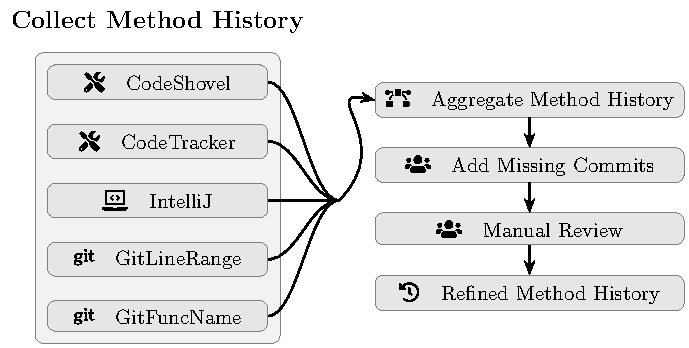
\includegraphics[width=\textwidth]{figure/method-history-refinement-process.pdf}
\caption{The process used to generate accurate oracles. The union of the change commits reported by all tools was first created, missing commits were added, and false positives were then removed.}
% \Description{The process to generate accurate oracles. We first took the union of the change commits reported by all tools, added missing commits, and then removed the false positives.}
\label{fig:oracle-construction-process}
\end{figure}

\subsection{Updating the CodeShovel Oracle}
\label{sec:updating-codeshovel-oracle}
Using the five tools (\textit{CodeShovel}, \textit{CodeTracker}, \textit{IntelliJ}, \textit{GitLineRange}, and \textit{GitFuncName}), method change histories were collected for the 200 methods used in the original \textit{CodeShovel} study. For \textit{CodeShovel} and \textit{CodeTracker}, the tools were used as library dependencies, as they are publicly available on \texttt{GitHub}. For \textit{IntelliJ}, each project was manually imported, the specific commits were checked out, the target files and methods were located, and the \texttt{Show History for Selection} option was used to generate the method change histories. For the Git-based tools, shell commands namely \texttt{git log <commit> --no-merges -L :<funcname>:<file>} and \texttt{git log <commit> --no-merges \allowbreak{}-L <start>,<end>:<file>} were executed to collect method histories. Finally, the method change histories from all five tools were aggregated into a unified commit history, producing a union of the commit histories of all tools. The missing commits mentioned earlier were also added. The commit histories were then sorted in reverse chronological order by their commit timestamp. Next, each method change commit was manually inspected to verify its logical validity by comparing it with its parent commit. This process is repeated iteratively for each subsequent commit until all commits have been thoroughly examined. At the end of this process, a complete and accurate method history oracle was obtained for the 200 methods. These 200 methods are referred to as the corrected \textit{CodeShovel} oracle.

\subsection{Constructing the HistoryFinder Oracle}
\label{sec:history-finder-oracle}
The \textit{HistoryFinder} oracle was created from 20 additional open-source Java projects selected from \texttt{GitHub}. To ensure high-quality projects~\cite{kalliamvakou_promises_2014}, popular projects were selected based on a high number of stars and forks. Each project was also required to have at least 2,000 commits so that enough method change commits could be found for the selected methods from these projects.
Table \ref{tab:history-finder-repository-list} presents the list of selected projects along with their number of commits, Java files, methods, and their respective star and fork counts. From each project, 10 methods were randomly selected, recording their file names, method names, and start and end line numbers, resulting in a total of 200 methods. The same approach described in section \ref{sec:updating-codeshovel-oracle} was then followed to generate the change history oracle for this new set of 200 methods.

\begin{table}[ht]
\centering
\caption{Overview of the 20 Java repositories used for the \textit{HistoryFinder} oracle, including commit counts, source files, methods, and popularity metrics (stars and forks).}
\label{tab:history-finder-repository-list}
\resizebox{\linewidth}{!}{%
\begin{tabular}{lrrrrr}
\toprule
\textbf{Repository} & \textbf{\# Commits} & \textbf{\# Files} & \textbf{\# Methods} & \textbf{\# Stars} & \textbf{\# Forks} \\
\midrule
    auto & 2,570 & 317 & 4,211 & 10,441 & 1,202 \\
    cassandra & 31,705 & 4,926 & 76,475 & 8,913 & 3,641 \\
    dagger & 5,592 & 1,436 & 8,043 & 17,467 & 2,019 \\
    dubbo & 9,428 & 3,713 & 28,365 & 40,581 & 26,442 \\
    fastjson & 7,216 & 2,997 & 19,239 & 25,761 & 6,498 \\
    glide & 3,395 & 724 & 8,804 & 34,718 & 6,128 \\
    guice & 2,444 & 615 & 6,981 & 12,521 & 1,673 \\
    Hystrix & 2,354 & 415 & 6,436 & 24,160 & 4,708 \\
    j2objc & 6,314 & 5,119 & 106,062 & 5,998 & 972 \\
    jenkins & 37,342 & 1,779 & 21,660 & 23,363 & 8,834 \\
    jmeter & 32,202 & 1,526 & 16,138 & 8,468 & 2,116 \\
    kafka & 20,356 & 4,632 & 62,991 & 29,077 & 14,030 \\
    MPAndroidChart & 2,074 & 223 & 2,447 & 37,694 & 9,027 \\
    netty & 19,625 & 1,973 & 22,902 & 33,578 & 15,974 \\
    pulsar & 20,639 & 4,153 & 44,183 & 14,323 & 3,601 \\
    rocketmq & 8,918 & 1,581 & 17,155 & 21,361 & 11,727 \\
    RxJava & 7,698 & 1,884 & 33,994 & 47,951 & 7,602 \\
    shardingsphere & 43,769 & 7,765 & 34,921 & 20,035 & 6,775 \\
    tomcat & 77,289 & 2,705 & 42,021 & 7,619 & 5,062 \\
    zxing & 3,816 & 499 & 3,293 & 32,923 & 9,365 \\
\bottomrule
\end{tabular}
}
\end{table}

\section{Developing the HistoryFinder Tool and Algorithm}
\label{sec:history-finder-algorithm}

The first, third, and fourth authors collaboratively designed the \textit{HistoryFinder} algorithm through multiple Zoom meetings. The first author has 8+ years of industry experience; the third has 14+ years in industry and 3+ in research; and the last has 1 year in industry and 15 years in research. During these sessions, they analyzed the strengths and limitations of two existing approaches, \textit{CodeShovel} and \textit{CodeTracker}, which guided the design of their new algorithm. Their analysis revealed that while \textit{CodeTracker} is generally more accurate than \textit{CodeShovel}, it suffers from significantly slower runtime performance. This is primarily due to its dependence on RefactorMiner, whereas \textit{CodeShovel} uses a simpler, faster string-matching algorithm. To balance accuracy and efficiency, \textit{HistoryFinder} adopts \textit{CodeShovel’s} lightweight string-matching approach but improves upon it with a more precise method-tracking strategy. The main algorithmic differences are as follows.
\begin{itemize}
    \item In Phase 2 of the \textit{CodeShovel} algorithm, the first method with body similarity $\ge0.75$ is selected, without checking for a matching signature. This can lead to tracking an extracted method instead of the original. In contrast, \textit{HistoryFinder} first checks for a matching signature and resorts to body similarity only if none is found.
\item When the method is not found in the same file, \textit{CodeShovel} performs two phases: first, it looks for methods with the same signature (even with low body similarity), then for methods with high body similarity. During the training phase, a method in a different file with the same signature but low similarity was observed to not necessarily be the same method. Merging these phases---directly searching for highly similar methods without checking the signature---improves precision.

\item Additionally, in Phase 4, \textit{CodeShovel} compares all methods across modified files, which is not only time-consuming but can also lead to incorrect matches, especially in the case of method overloading. This issue was addressed by filtering out methods that were unchanged in both commits, as such methods cannot be the ones of interest. Also, \textit{CodeShovel} returns the first score exceeding the threshold, which is problematic when a more similar method exists. To alleviate this issue, \textit{HistoryFinder} returns the best matching method passing the similarity threshold.
\end{itemize}

\textit{HistoryFinder} also improved some of the technical weaknesses that \textit{CodeShovel} has. For example, during development, if code is merged without rebasing, conflicts can arise when a method is modified concurrently in different branches. The resolution of these conflicts may introduce changes to the method’s history that must be considered. \textit{CodeShovel}, however, excludes merge commits and ignores changes introduced during merges. In this approach, merge commits are included, and the method’s state is compared with each parent commit, allowing accurate detection of any changes introduced from either parent branch. Moreover, \textit{CodeShovel} does not account for formatting changes, annotation, or JavaDoc updates, whereas \textit{HistoryFinder} does. Another limitation of \textit{CodeShovel} is its case-insensitive string-matching algorithm. This approach can be problematic, especially when comparing quoted string literals within a method body, as it may overlook subtle but important differences that could influence the method's behavior.

\subsection{Overview of HistoryFinder}
The \textit{HistoryFinder} tool needs several key inputs to trace the history of a method. These include the \texttt{Git} repository URL or local directory, a specific commit hash (SHA), the file path of the method (including the file name), the name of the method, and the line number where the method declaration begins. The output is a sequential list of commit hashes, each accompanied by relevant metadata. This metadata provides granularity of changes, such as changes to the method signature, body, and annotations, and identifies the contributor responsible for each modification. When executed via the command line, the output is saved as a \texttt{JSON} file.

The implementation utilizes the \texttt{JGit} library\footnote{https://github.com/eclipse-jgit/jgit last accessed: Jul 01, 2025}—a \texttt{Java}-based \texttt{Git} implementation—for repository cloning, commit traversal, and fine-grained file operations, including detection of added, deleted, moved, and modified files across revisions, and employs \texttt{JavaParser}\footnote{https://github.com/javaparser/javaparser last accessed: Jul 01, 2025} to generate an Abstract Syntax Tree (AST). Once the AST is constructed, it allows traversal through the list of methods in the file and extraction of specific components, such as the method signature, body, annotation, and JavaDoc. For method comparison, the implementation uses the Jaro-Winkler edit distance~\cite{winkler90} score similarity, as in \textit{CodeShovel}, between method signatures and bodies. Although \texttt{SimHash}~\cite{charikar_similarity_2002} was also tested for similarity matching, Jaro-Winkler consistently provides better recall than \texttt{SimHash}.

When the commit history is interpreted as a hierarchical graph structure, all commits leading up to a specific point in a \texttt{Git} project form a Directed Acyclic Graph (DAG)~\cite{geisshirt_git_2018}, representing the project's complete commit history to that point. To identify all commits that modified a method up to a given version (e.g., the starting commit), the DAG is traversed backward—from the target commit to its ancestors—until the commit where the method was originally introduced is reached. During this traversal, if a commit has a single parent, the method in the current commit is compared with its counterpart in the parent commit to detect changes. In the case of merge commits with multiple parents, the method may exist in any of the parent commits. Given that a project may contain thousands of commits (as shown in Table~\ref{tab:history-finder-repository-list}), traversing the entire DAG can be time-consuming. To optimize this process, \textit{HistoryFinder} leverages the \texttt{git log <commit> <file>} command, which filters the commit history to only those that modified the file containing the target method. This significantly reduces the search space, allowing traversal of a lightweight, file-specific DAG to detect method changes efficiently. However, if the method has been moved to a different file or the file itself has been renamed, a new DAG must be reconstructed from that point onward using the new file path.

\subsection{The HistoryFinder Algorithm}
Algorithm~\ref{alg:algorithm-history-finder} outlines how the file-specific DAG is constructed and traversed to detect the change history of a method. The procedure \textit{HistoryFinder} is initially invoked with the starting commit, file path, method name, and its starting line number. It may be invoked recursively if the method is detected to have moved to a different file or if the file itself has been renamed. To build the DAG, the utility procedure \textit{GITLOG} is first called (line 2), which internally executes the \texttt{git log <commit> <file>} command. This retrieves only the commits that have modified the target file containing the method. Using these filtered commits, a directed acyclic graph \( G \) is constructed, where each node represents a commit that changed the file. In the DAG, an edge is drawn from node $u$ to node $v$ if the file is modified in commit $u$, followed by in commit $v$, establishing a direct connection between them. Once the DAG is constructed, it is traversed using the Breadth-First Search (BFS) algorithm~\cite{cormen_introduction_2022} to systematically explore all relevant commits.

Queue \( Q \) keeps track of all discovered commit nodes that need to be explored. To unambiguously locate the target method in a commit, each commit node is represented by a structure containing the commit hash, file path, method name, and line number, created by invoking \texttt{Create} (line 3 for the initial node) procedure. The queue \( Q \) is initialized with the starting node (line 4), which is also the only entry in the set \texttt{visited} to mark it as explored. Whenever a change to the method is detected, it is recorded in the history list \( H \), which is initially empty (line 6). The \texttt{while} loop iterates through all discovered nodes. In each iteration, an unexplored commit node \( u \) is dequeued from the head of \( Q \) (line 8). The method already found in commit node \( u \) is located by calling the procedure \texttt{Find} (line 9), which takes the commit hash, file, method name, and line number as parameters, accessed using dot notation. Next, the parent node \( p \) of \( u \) is retrieved (line 10), where the method might be found. From lines 11 to 18, the algorithm checks whether the method exists in the direct parent commit \( p \), accounting for possible modifications.

\begin{algorithm}
\caption{HistoryFinder Algorithm}
\label{alg:algorithm-history-finder}
\footnotesize
\SetKwFunction{hf}{HistoryFinder}
\SetKwProg{Procedure}{procedure}{:}{end procedure}

\Procedure{\hf{$hash,file,name,line$}}{ %\tcp*[r]{$name$ and $line$ are the method's name and start line}
    
    \KwIn{
      $hash$: Start commit hash\linebreak
      \Indp
        $file$: File containing the method\linebreak
        $name$: Method name\linebreak
        $line$: Start line of the method
      \Indm
    }
    \KwOut{Change history of the input method}
    $G \gets \textsc{GitLog}(hash, file)$\tcp*[r]{Build file-level DAG}
    $s \gets \textsc{Create}(hash,file,name,line)$\;
    $Q \gets \{s\}$\tcp*[r]{Initialize queue with start node}
    
    $visited \gets \{s\}$\tcp*[r]{Track visited nodes}
    $H \gets \emptyset$\tcp*[r]{Initialize with empty method history}
    \While{$Q \neq \emptyset$}{ %\tcp*[r]{Process all discovered commit nodes}
        $u \gets \textsc{Dequeue}(Q)$\;
        $um \gets \textsc{Find}(u.hash, u.file, u.name, u.line)$\;
        $p \gets \textsc{Parent}(G, u)$ \tcp*[r]{Direct parent commit}
        \BlankLine
        \tcp{Search method by signature, body in original file, then body in other files}
        $m \gets \textsc{SignatureMatch}(p,file,um)$\;
        $altFile \gets \textsc{NIL}$\tcp*[r]{Track method/file move}
         \If{$m == \text{NIL}$}{ %\tcp*[r]{No match by signature}
            $m \gets \textsc{BodyMatch}(p,file,um, 0.70)$\;
            \If{$m == \text{NIL}$}{%\tcp*[r]{No match by body similarity}
                %\tcp*[r]{Examine other files}
                $m,altFile \gets \textsc{AltFileMatch}(u.hash,p,um)$;
            }
        }
        \BlankLine
        \tcp{Method found in original/other file}
        \If{$m \not= \text{NIL}$}{
            \If{$um.\text{text} \not= m.\text{text} \textbf{ or } altFile \not= \textsc{NIL}$}{
                \textsc{Add}$(H, u)$ \tcp*[r]{Record method change}
            }
            \tcp{Continue tracking in the new file}
            \If{$altFile \not= \textsc{NIL}$}{% \tcp*[r]{Method or file moved}
                $sH \gets \textsc{HistoryFinder}(m.hash,m.file,m.name,m.line)$\;
                %\vspace{-0.35cm}
                \textsc{AddAll}$(H, sH)$ \tcp*[r]{Append sub-history}
            }
        \tcp{Enqueue unvisited ancestor commits}
        \If{$m \not= \textsc{NIL} \textbf{ and } altFile == \textsc{NIL}$}{ %\tcp*[r]{Method remained in the same file}
            \ForEach{$v \in G.\text{Adj}[u]$}{
                \If{$v \notin visited$}{
                    \textsc{Add}$(visited, v)$\;
                    $v.name \gets m.name$\;
                    $v.line \gets m.line$\;
                    \textsc{Enqueue}$(Q, v)$\;
                }
            }
        }
        }
    }    
    \Return $H$\;
}
\end{algorithm}

\begin{algorithm}
\caption{Utility Procedures for Method Matching}
\label{alg:history-finder-similarity-matching}
% \small
\footnotesize
\SetKwFunction{fbsm}{SignatureMatch}
\SetKwFunction{fbbm}{BodyMatch}
\SetKwFunction{afm}{AltFileMatch}
\SetKwProg{Procedure}{procedure}{:}{end procedure}
\Procedure{\fbsm{$hash,file,tm$}}{%\tcp*[r]{Match target method by exact signature}
    \KwIn{
      $hash$: Commit hash\linebreak
      \Indp
        $file$: File containing methods\linebreak
        $tm$: Target method
      \Indm
      }
    \KwOut{Matching method or $\text{NIL}$ if not found}
    $methods \gets \textsc{ParseMethod}(hash, file)$\;%\tcp*[r]{Parse methods}
    \ForEach{$m \in methods$}{%\tcp*[r]{Iterate through parsed methods}
        %\tcp*[h]{Match signature}\;
        \If{$m.\text{signature} == tm.\text{signature}$}{
            \Return $m$ \tcp*[r]{Return matching method}
        }
    }
    \Return $\text{NIL}$ \tcp*[r]{No matching method found}
}
\BlankLine
%\tcp*[r]{Match target method by body similarity}
\Procedure{\fbbm{$hash,file, tm, threshold$}}{% \tcp*[r]{Match target method by body similarity}
    \KwIn{
      $hash$: Commit hash\linebreak
      \Indp
        $file$: File containing methods\linebreak
        $tm$: Target method\linebreak
        $threshold$: Similarity threshold for matching
      \Indm
      }
    \KwOut{
    $bm$: Best matching method meeting threshold\linebreak
      \Indp
        $bs$: Similarity score of the best match
      \Indm}
    $methods \gets \textsc{ParseMethod}(hash, file)$\; %\tcp*[r]{Parse methods}
    $bm \gets \text{NIL}$ \tcp*[r]{Initialize best matching method}
    $bs \gets 0$ \tcp*[r]{Initialize highest similarity score}
    \ForEach{$m \in methods$}{% \tcp*[r]{Iterate through all methods}
        %\tcp{Compute similarity with target method}
        $score \gets \textsc{Similarity}(m.text,tm.text)$\;
        \If{$score >= threshold \textbf{ and } score > bs$}{
            $bm \gets m$ \tcp*[r]{Update best matching method}
            $bs \gets score$ \tcp*[r]{Update highest similarity}
        }
    }
    \Return $bm,bs$\;
}
\BlankLine
\Procedure{\afm{$hash,parentHash,tm$}}{% \tcp*[r]{Search for target method in other modified files}
   \KwIn{
      $hash$: Commit hash\linebreak
      \Indp
        $parentHash$: Parent commit hash\linebreak
        $tm$: Target method
      \Indm
      }
    \KwOut{
    $bm$: Best matching method\linebreak
      \Indp
        $altFile$: File containing the best matching
      \Indm}
    %\tcp{Get files changed between commits}
    $changeFiles \gets \textsc{findChangeFiles}(hash,parentHash)$\;
    $bm \gets \text{NIL}$ \tcp*[r]{Initialize best matching method}
    $bs \gets 0$ \tcp*[r]{Initialize highest similarity score}
    $altFile \gets \textsc{NIL}$ \tcp*[r]{Best method matching file}
    \ForEach{$file \in changeFiles$}{
        $m,s \gets \textsc{BodyMatch}(parentHash,file,tm,0.75)$\;
        \If{$s > bs$}{%\tcp*[r]{Update best match if score improves}
            $bm \gets m$\;
            $bs \gets s$\;
            $altFile \gets file$\;
        }
    }
    \Return $bm,altFile$\;
}
\end{algorithm}

The algorithm first tries to locate the method by matching its signature (line 11), including the method name and parameters, but excluding the return type. If the signature match fails, it attempts to locate the method by the textual similarity of its body (line 14), considering a match valid if the similarity is at least 70\%. If the method still cannot be found, the search expands to other modified files (line 16), raising the similarity threshold to 75\% in this case. If the method is found in a different file—due to a method move or a file rename/move—the new file path is recorded in \texttt{altFile}. When the method is located through any of the above mechanisms (line 19), the algorithm checks whether the methods (from the current and parent commits) are identical, including their signatures, JavaDocs, annotations, or whether the file has been renamed or moved (in which case \texttt{altFile} should not be \texttt{NIL}) (line 20). If any change is detected—either in the method or in the file name or path—this change is recorded by invoking the \texttt{Add} procedure (line 21).

If the method is found in another file, a new DAG must be reconstructed for that file. To do so, the \texttt{HistoryFinder} procedure is recursively called (line 24), returning a sub-history that is appended to \( H \) (line 25). If the method is instead found within the same file (line 27), all immediate ancestor commit nodes are processed. In this case, all adjacent ancestor commit nodes of \( u \) that have not yet been visited are added to the visited set (line 30) and enqueued (line 33). The method name (line 31) and line number (line 32) are also updated to reflect the newly found version, so that it can be retrieved accurately when this node is dequeued later. Once all nodes have been processed, the resulting sequence of commit nodes captures the method’s change history in \(H\). Additionally, the furthest node dequeued from the queue $Q$ is added as the introduction commit, since this is the earliest known instance of the method.

Algorithm~\ref{alg:history-finder-similarity-matching} defines the utility procedures used to compare and match methods based on textual similarity. The procedure \texttt{SignatureMatch} attempts to locate the target method within a Java file at a specific commit. Line 2 parses all methods in the file using \texttt{JavaParser}, and lines 3 to 7 iterate over these methods, comparing each one’s signature with the target method. If a matching signature is found, the corresponding method is returned (line 5); otherwise, \texttt{NIL} is returned (line 8). The next procedure, \texttt{BodyMatch} (line 10), identifies a method based on the highest body similarity with the target method, provided it exceeds a specified similarity threshold. A threshold of 70\% is used when comparing methods within the same file, and 75\% when comparing across different files. Line 11 parses all Java methods in the file provided as input. The variable \texttt{bm} (line 12) tracks the best matching method, while \texttt{bs} (line 13) stores the corresponding similarity score. Line 14 iterates over all parsed methods, and the \texttt{Similarity} procedure (line 15) computes the similarity between the current method and the target method using the Jaro-Winkler algorithm~\cite{winkler90}. If the computed similarity meets the threshold and is greater than the current best score \texttt{bs}, both the score and the best matching method are updated (lines 16–19). Finally, the best matching method along with its similarity score is returned (line 21).

The procedure \texttt{AltFileMatch} attempts to locate the target method in all files that were modified in a given commit. It begins by listing all modified files using the \texttt{FindChangedFiles} procedure (line 24). Lines 25 to 27 initialize variables to track the best matching method, its similarity score, and the corresponding file path. Each modified file is then iterated (line 28), and the best matching method within each file is identified (line 29). If a method with a higher similarity score is found, the method information is updated accordingly (lines 30–34). Finally, the method with the highest similarity score and the new file path are returned (line 36). Similar to the \textit{CodeShovel} algorithm~\cite{grund_codeshovel_2021}, the first 100 methods from the corrected \textit{CodeShovel} oracle were used to train the algorithm and determine the optimal thresholds for body similarity within the original and other files.

\section{Analysis and Results}
\label{sec:result-and-analysis}
This section compares the corrected \textit{CodeShovel} oracle with the original \textit{CodeShovel} and \textit{CodeTracker} oracles. It then evaluates the accuracy and runtime efficiency of all method change history generation tools using the corrected \textit{CodeShovel} and the newly developed \textit{HistoryFinder} oracles. In particular, it answers the following three research questions.
\begin{itemize}
    \item \textbf{RQ1}: To what extent does the corrected \textit{CodeShovel} oracle differ from the original oracles?
    \item \textbf{RQ2}: Which history generation tool exhibits the highest accuracy when evaluated with the two new oracles?
    \item \textbf{RQ3}: Which history generation tool exhibits the best runtime performance?
\end{itemize}
\subsection{RQ1: Difference with the corrected CodeShovel oracle}

After correcting the 200 method histories in both the \textit{CodeShovel} and \textit{CodeTracker} oracles, the new systematically constructed oracle—\emph{the corrected CodeShovel oracle}—was compared with the original \textit{CodeShovel} and \textit{CodeTracker} oracles, revealing significant updates. Table~\ref{tab:oracle-update-statistics} provides a detailed breakdown of the changes. It shows how many methods were \emph{changed}, commits were \emph{added}, and \emph{removed}. A method is considered \emph{changed} if the new oracle has a different set of commits than the original. A commit is considered \emph{added} if it was not present in the original oracles, and \emph{removed} if it was inaccurately included. For example, the last column shows that the \textit{CodeTracker} oracle has fewer inaccurate commits (67) than the original \textit{CodeShovel} oracle. In contrast, it missed many commits that should have been recorded as change commits for those 200 methods, as shown in the \emph{\# Added} column.

Compared to the original \textit{CodeShovel} oracle, the histories of 40 methods were \emph{modified}, with 59 commits \emph{added} and 186 \emph{removed}. These changes exclude annotations, JavaDocs, and formatting—omitted by the original \textit{CodeShovel} and \textit{CodeTracker} oracles, though \textit{CodeTracker} did include annotations. When these types of changes were included, 142 method histories were affected, and 429 commits were \emph{added}. Significant changes were also observed when compared with the \textit{CodeTracker} oracle. These changes suggest that the previous evaluations of method tracing tools (e.g., \textit{CodeShovel} and \textit{CodeTracker}) may not reflect the true precision and recall of these tools in tracing a method's change history.


\begin{table}[t]
\centering
\caption{Comparison between the corrected and original oracles. As the corrected oracle includes changes related to annotations, JavaDocs, and formatting, the differences are shown both including (\emph{Incl.}) and excluding (\emph{Excl.}) those changes.}
\label{tab:oracle-update-statistics}
% \resizebox{\linewidth}{!}{%
\begin{tabular}{lrrrrr}
\toprule
\multirow{3}{*}{\textbf{Oracle}}

& \multicolumn{2}{c}{\textbf{\# Methods}} & \multicolumn{3}{c}{\textbf{\# Commits}}\\
\cmidrule(lr){2-3} \cmidrule(lr){4-6}

& \multicolumn{2}{c}{\textbf{\# Changed}} & \multicolumn{2}{c}{\textbf{\# Added}} & \textbf{\# Removed} \\
 & \textbf{Incl.} & \textbf{Excl.} & \textbf{Incl.} & \textbf{Excl.} & \\
\cmidrule(lr){1-1} \cmidrule(lr){2-3} \cmidrule(lr){4-6}
CodeShovel & 142 & 40 &  429 & 59 & 186 \\
CodeTracker & 133 & 43 &  445 & 134 & 67 \\
\bottomrule
\end{tabular}
% }
\end{table}



To illustrate inaccuracies in both the \textit{CodeShovel} and \textit{CodeTracker} oracles, several cases are highlighted. One representative example is the \texttt{fireErrors} method from the \texttt{checkstyle} project. Both the \textit{CodeShovel}\footnote{\href{https://github.com/SQMLab/HistoryFinder/blob/main/oracle/codeshovel-oracle/checkstyle-Checker-fireErrors.json}{https://github.com/SQMLab/HistoryFinder/blob/main/oracle/codeshovel-oracle/checkstyle-Checker-fireErrors.json}} and \textit{CodeTracker}\footnote{\href{https://github.com/SQMLab/HistoryFinder/blob/main/oracle/codetracker-oracle/checkstyle-Checker-fireErrors.json}{https://github.com/SQMLab/HistoryFinder/blob/main/oracle/codetracker-oracle/checkstyle-Checker-fireErrors.json}} oracles record this method’s history beginning from commit \texttt{119fd4}, where the method resided in \path{src/main/java/com/puppycrawl/tools/checkstyle/Checker.java}. However, both oracles incorrectly identified commit \texttt{0e3fe} as the method’s introduction, whereas it was actually introduced earlier in commit \texttt{0fd69} (the method name was \texttt{displayErrors} and was later renamed to \texttt{fireErrors}). This error was recently corrected in the \textit{CodeTracker} oracle; however, the evaluation was conducted using the original published version, where the issue was present.

In another case (\texttt{createPattern method}) in the \textit{CodeShovel} oracle\footnote{\href{https://github.com/checkstyle/checkstyle/compare/d2551035044a845fd1b3e345f2470875a43a8991...f2c6263e151e8a7300755b36fbb41511c0a0cca1\#diff-1b66e778c19cac5ac2beaec4d6a74c8c37a5fd83d39db4bef8c1b60b9ec68c0e}{https://github.com/checkstyle/checkstyle/compare/d2551035044a845fd1b3e345f2470875a43a8991...\allowbreak f2c6263e151e8a7300755b36fbb41511c0a0cca1\#diff-1b66e778c19cac5ac2beaec4d6a74c8c37a5fd83d39db4bef\allowbreak 8c1b60b9ec68c0e last accessed: July 3, 2026}}, while saving the history of an overloaded method, the history failed to stop at the point where the overloaded method was introduced and inaccurately switched to tracing the original of the overloaded method, resulting in incorrect method changes in the oracle. Another challenge arises when handling merge commits. While the \textit{CodeShovel} oracle completely ignored changes that occurred in merge commits, the \textit{CodeTracker} oracle occasionally added incorrect method changes. An example of this issue occurs in the \texttt{runChild} method of the \texttt{junit4} project. Although the diff\footnote{\href{https://github.com/junit-team/junit4/compare/8ff0b44e3fb0c1c56a1dc6290c3b6828a5a8f9bf...bed58a573c373d57d64fa369f58b2a8f0dbee3d7\#diff-cd3bb9170f8d6404c5dc5bb66f7b647435854d48fe357e0bd998e3011a575929}{https://github.com/junit-team/junit4/compare/8ff0b44e3fb0c1c56a1dc6290c3b6828a5a8f9bf...\allowbreak bed58a573c373d57d64fa369f58b2a8f0dbee3d7\#diff-cd3bb9170f8d6404c5dc5bb66f7b647435854d48fe357e0bd\allowbreak998e3011a575929 last accessed: July 3, 2026}} appears to show a method change, it is incorrect—the commit has two parents,\footnote{\href{https://github.com/junit-team/junit4/blob/a49240ade1974b948b20cf2c45d9129f04122735/src/main/java/org/junit/runners/BlockJUnit4ClassRunner.java\#L64}{https://github.com/junit-team/junit4/blob/a49240ade1974b948b20cf2c45d9129f04122735\allowbreak/src/main/java/org/junit/runners/BlockJUnit4ClassRunner.java\#L64 last accessed: July 3, 2026}} and the comparison was made against the wrong parent.\footnote{\href{https://github.com/junit-team/junit4/blob/708ed373c02b467422890d5163fff46d1f32ab01/src/main/java/org/junit/runners/BlockJUnit4ClassRunner.java\#L66}{https://github.com/junit-team/junit4/blob/708ed373c02b467422890d5163fff46d1f32ab01\allowbreak/src/main/java/org/junit/runners/BlockJUnit4ClassRunner.java\#L66 last accessed: July 3, 2026}} In reality, the code was introduced from the other branch\footnote{\href{https://github.com/junit-team/junit4/blob/9d8bb069f68e2194db742981972c8930381b62c2/src/main/java/org/junit/runners/BlockJUnit4ClassRunner.java\#L65}{https://github.com/junit-team/junit4/blob/9d8bb069f68e2194db742981972c8930381b62c2\allowbreak/src/main/java/org/junit/runners/BlockJUnit4ClassRunner.java\#L65 last accessed: July 3, 2026}} without any modification.

\begin{framed}
\noindent\textbf{\underline{RQ1 summary}:}
Both the \textit{CodeShovel} and \textit{CodeTracker} oracles contain inaccuracies in their constructed method histories. The updated, more accurate oracle can serve as a valuable resource for effectively evaluating both existing and future method-level change history generation tools.
\end{framed}

\subsection{RQ2: Accuracy of the change history generation tools}
\label{sec:rq2-accuracy}
The accuracy of six method change history generation tools, including the newly proposed \textit{HistoryFinder}, is evaluated next. This evaluation uses the corrected \textit{CodeShovel} oracle (200 methods) and the new \textit{HistoryFinder} oracle (another 200 methods). The \textit{CodeShovel} oracle is divided into two parts: \textit{CodeShovel Training} and \textit{Testing} oracles. This distinction is important, as both the \textit{CodeShovel} and \textit{HistoryFinder} algorithms were trained and tuned using the training portion of the \textit{CodeShovel} oracle. The three research-based tools were run as Java libraries to extract method histories and compute accuracy metrics. For Git-based tools, the command \texttt{git log <commit> --no-merges -L :<funcname>:<file>} was used to generate method histories for \textit{GitFuncName}, which tracks changes by function name, and \texttt{git log <commit> --no-merges\allowbreak{} -L <start>,\allowbreak{}<end>:<file>} was used for \textit{GitLineRange}, which tracks changes by line range. In contrast, for \textit{IntelliJ}, IntelliJ IDEA 2024.3 Community Edition was used to manually generate method histories (\texttt{Right-click} $\rightarrow$ \texttt{Git} $\rightarrow$ \texttt{Show History for Selection}), as no automated approach exists for running IntelliJ's method tracking feature.

Precision, recall, and F1 score were calculated for all the tools against the three oracles. Since tools differ in the types of changes they detect (e.g., \textit{CodeShovel} ignores annotations, \textit{CodeTracker} ignores formatting), the expected commit sets were tailored to match each tool’s capabilities, ensuring a fair and meaningful comparison. The tools' accuracy is evaluated at two granularities: \emph{commit-level} and \emph{method-level}. At the \emph{commit-level}, precision, recall, and F1 scores are computed by aggregating true positives (TP), false positives (FP), and false negatives (FN) across each oracle, based on the total expected commits. At the \emph{method-level}, metrics are computed per method and averaged across each oracle.

\begin{table*}[t]
\centering
\caption{Precision, recall, and F1 score for method history tracking tools across three oracles.
\textbf{TP} (True Positives) indicates correctly identified change commits;
\textbf{FP} (False Positives) refers to incorrectly included commits;
\textbf{FN} (False Negatives) denotes missed commits that should have been identified. \textbf{Bolded values indicate the best performance in each metric within an oracle.}}
\label{tab:hf-method-tracking-score}
\resizebox{\textwidth}{!}{%
% \small
% \setlength{\tabcolsep}{3pt}
\begin{tabular}{llrrrrrrrrr}
\toprule
\multirow{2}{*}{\textbf{Oracle}} & \multirow{2}{*}{\textbf{Tool}} & \multicolumn{6}{c}{\textbf{\emph{Commit-Level}}} & \multicolumn{3}{c}{\textbf{\emph{Method-Level}}} \\
\cmidrule(lr){3-8} \cmidrule(lr){9-11}
 &  & \textbf{TP} & \textbf{FP} & \textbf{FN} & \textbf{Precision} & \textbf{Recall} & \textbf{F1} & \textbf{Precision} & \textbf{Recall} & \textbf{F1} \\

\cmidrule(lr){1-1} \cmidrule(lr){2-2} \cmidrule(lr){3-5}  \cmidrule(lr){6-8} \cmidrule(lr){9-11}

\multirow{6}{*}{CodeShovel Training}
    & CodeShovel & 2813 & 158 & 28 & 94.68 & \textbf{99.01} & 96.80 & 94.79 & \textbf{99.31} & 95.86 \\
    & CodeTracker & 2804 & 32 & 76 & 98.87 & 97.36 & 98.11 & 98.99 & 96.98 & 97.52 \\
    & HistoryFinder & 3047 & 6 & 67 & \textbf{99.80} & 97.85 & \textbf{98.82} & \textbf{99.68} & 98.15 & \textbf{98.53} \\
    & IntelliJ & 2146 & 402 & 919 & 84.22 & 70.02 & 76.47 & 85.16 & 75.08 & 73.40 \\
    & GitLineRange & 2197 & 1135 & 787 & 65.94 & 73.63 & 69.57 & 77.94 & 76.32 & 68.29 \\
    & GitFuncName & 1749 & 1166 & 1261 & 60.00 & 58.11 & 59.04 & 72.93 & 62.03 & 54.88 \\
\cmidrule(lr){1-1} \cmidrule(lr){2-2} \cmidrule(lr){3-5}  \cmidrule(lr){6-8} \cmidrule(lr){9-11}
\multirow{6}{*}{CodeShovel Testing}
    & CodeShovel & 812 & 25 & 38 & 97.01 & 95.53 & 96.27 & 97.40 & 95.70 & 95.54 \\
    & CodeTracker & 811 & 35 & 63 & 95.86 & 92.79 & 94.30 & 97.59 & 94.36 & 94.76 \\
    & HistoryFinder & 938 & 10 & 7 & \textbf{98.95} & \textbf{99.26} & \textbf{99.10} & \textbf{99.15} & \textbf{99.24} & \textbf{99.15} \\
    & IntelliJ & 685 & 239 & 249 & 74.13 & 73.34 & 73.74 & 85.14 & 72.58 & 73.78 \\
    & GitLineRange & 609 & 288 & 279 & 67.89 & 68.58 & 68.24 & 87.48 & 70.02 & 72.31 \\
    & GitFuncName & 579 & 393 & 331 & 59.57 & 63.63 & 61.53 & 77.85 & 65.34 & 65.35 \\
\cmidrule(lr){1-1} \cmidrule(lr){2-2} \cmidrule(lr){3-5}  \cmidrule(lr){6-8} \cmidrule(lr){9-11}
\multirow{6}{*}{HistoryFinder}
    & CodeShovel & 2095 & 147 & 394 & 93.44 & 84.17 & 88.56 & 95.68 & 86.45 & 85.82 \\
    & CodeTracker & 2354 & 88 & 168 & \textbf{96.40} & 93.34 & 94.84 & 94.43 & 91.24 & 94.14 \\
    & HistoryFinder & 2835 & 106 & 48 & \textbf{96.40} & \textbf{98.34} & \textbf{97.36} & \textbf{96.49} & \textbf{96.81} & \textbf{97.00} \\
    & IntelliJ & 2185 & 1530 & 637 & 58.82 & 77.43 & 66.85 & 75.99 & 81.38 & 75.80 \\
    & GitLineRange & 2032 & 2112 & 616 & 49.03 & 76.74 & 59.84 & 77.64 & 82.98 & 75.50 \\
    & GitFuncName & 1858 & 2638 & 835 & 41.33 & 68.99 & 51.69 & 65.08 & 72.67 & 59.50 \\
\bottomrule
\end{tabular}
}
\end{table*}

Table~\ref{tab:hf-method-tracking-score} shows that all research-based tools—\textit{CodeShovel}, \textit{CodeTracker}, and \textit{HistoryFinder}—significantly outperform \textit{IntelliJ} and \texttt{Git-based} tools. Overall, \textit{HistoryFinder} achieves the highest F1 score. In terms of precision, \textit{HistoryFinder} and \textit{CodeTracker} slightly outperform \textit{CodeShovel}. For recall, \textit{CodeShovel} performs best on its own training oracle; however, on the other two oracles, \textit{HistoryFinder} achieves the highest recall. \textit{CodeShovel’s} notably lower recall on the \textit{HistoryFinder} oracle is primarily due to its failure to generate the complete history for several methods. For example, it was unable to produce complete histories for all 10 methods from the Cassandra project. Additionally, it failed entirely for two methods in the Fastjson project due to \texttt{JavaParser} errors that prevented successful file parsing. Overall, across all three oracles, \textit{HistoryFinder} demonstrates the most consistent and superior performance. Results at the \emph{method-level} scores closely correlate with \emph{commit-level} scores, with minor variations. For instance, \textit{CodeShovel's} precision against the \textit{HistoryFinder} oracle is approximately 2\% higher at the \emph{method-level} compared to the \emph{commit-level}.
The Wilcoxon rank-sum test~\cite{wilcoxon_individual_1945} also shows that the observed accuracy gain with \textit{HistoryFinder} is statistically significant ($P \le 0.05$).

\begin{framed}
\noindent\textbf{\underline{RQ2 summary}:}
The \textit{HistoryFinder} algorithm consistently achieves the highest precision and F1 score in change history detection. Between \textit{CodeShovel} and \textit{CodeTracker}, performance varies depending on the scenario. Notably, \textit{CodeShovel's} recall drops significantly on the entirely new oracle of 200 methods, mainly because it fails to generate the full or any history for a subset of methods. Given these findings, researchers or practitioners who prioritize accuracy should consider \textit{HistoryFinder} the most reliable option.
\end{framed}

\subsection{RQ3: Runtime performance of the change history generation tools}
\label{sec:rq3-runtime}

The tools were executed in a controlled environment on a machine equipped with \emph{32GB of RAM, an Intel(R) Core(TM) i7-8700 CPU @ 3.20GHz with 12 cores, running Ubuntu 22.04 LTS and Java 21 x86}. Execution time for \textit{IntelliJ} was not recorded since method histories were generated manually from \texttt{IntelliJ IDEA}, making it infeasible to measure the time. Prior to recording execution time, all repositories were cloned to a local persistent storage. Initially, the JAR dependencies of the research-based tools were integrated. However, caching of parsed Java files across multiple method history runs—particularly in \textit{CodeShovel}—was observed to significantly reduce the runtime. While this optimization benefits batch processing, it does not yield deterministic or representative runtimes for tracing individual methods. To ensure a fair comparison, each tool was instead executed independently for each method history using the \texttt{java -jar} command. This approach ensured that each method's history was processed in isolation within a fresh environment, by launching a separate \texttt{JAR} process for each run and terminating it upon completion. Please note that due to the deterministic nature of the evaluated tools, the difference in execution times in multiple runs for a given tool is negligible.

\begin{figure*}[t]
  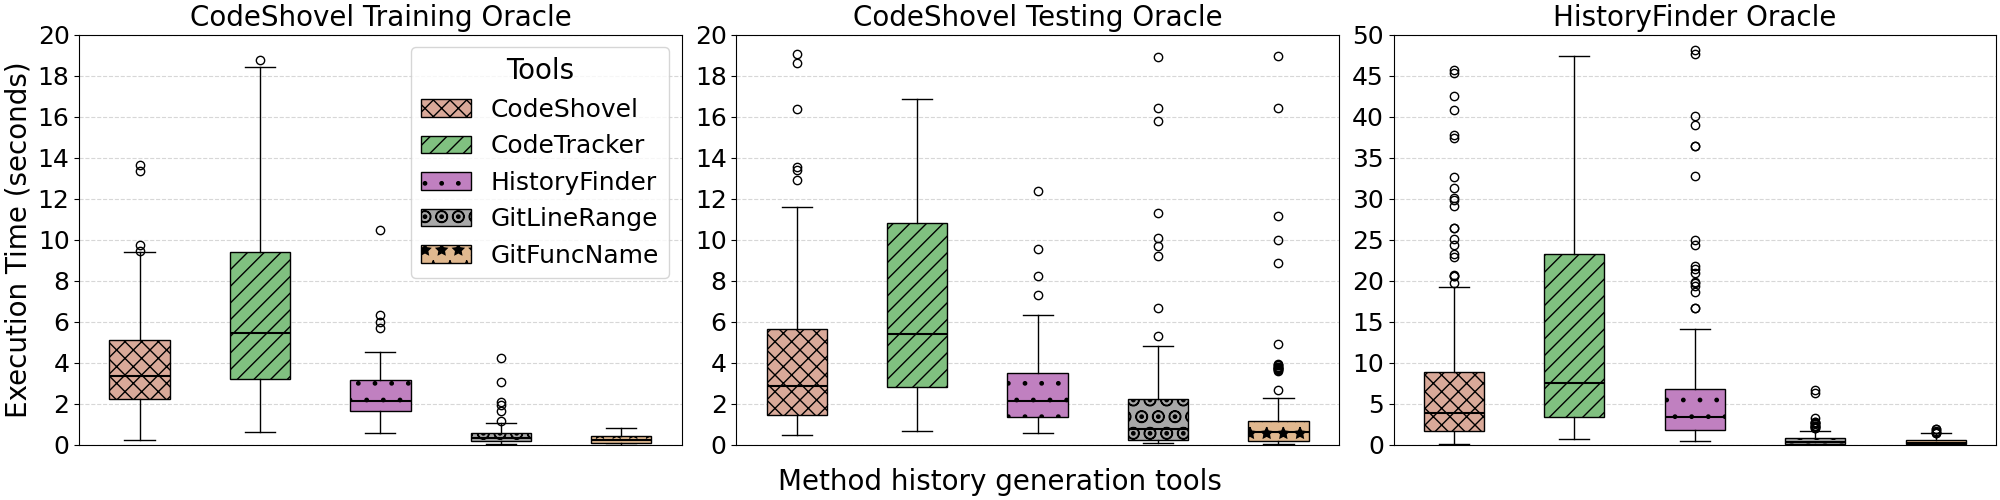
\includegraphics[width=\linewidth]{figure/execution-time-box-plot.png}
\caption{Comparison of execution times across three oracles for five tools. To enhance readability, the y-axis is limited to 20 seconds for the first two subplots (\textit{CodeShovel} oracles) and 50 seconds for the third subplot (\textit{HistoryFinder} oracle).}
% \Description{Comparison of execution times across three oracles for five tools. To enhance readability, the y-axis is limited to 20 seconds for the first two subplots (\textit{CodeShovel} oracles) and 50 seconds for the third subplot (\textit{HistoryFinder} oracle).}
\label{fig:execution-time-box-plot}
\end{figure*}



\begin{table}[ht]

\centering
\caption{Execution times (in seconds) for the five tools. \textit{IntelliJ} is excluded because of the need for manual execution.}
% \Description{Mean, median, minimum, and maximum execution times (in seconds) for five tools.
% \textbf{Bold} values indicate the best (lowest) execution time for both research-based and \texttt{Git}-based tools. \textit{IntelliJ} is excluded because method histories for this tool were generated manually using the \texttt{IDEA} interface.}
% \resizebox{\linewidth}{!}{%
\begin{tabular}{llrrrr}
\toprule
\textbf{Oracle} & \textbf{Tool} & \textbf{Mean} & \textbf{Median} & \textbf{Min} & \textbf{Max} \\ \midrule
\multirow{5}{*}{\makecell{CodeShovel\\Training}}
    & CodeShovel & 3.93 & 3.38 & \textbf{0.22} & 13.63 \\
    & CodeTracker & 8.71 & 5.45 & 0.64 & 76.80 \\
    & HistoryFinder & \textbf{2.51} & \textbf{2.15} & 0.59 & \textbf{10.48} \\
    \cmidrule(lr){2-2} \cmidrule(lr){3-6}
    & GitLineRange & 0.50 & 0.35 & 0.07 & 4.23 \\
    & GitFuncName & \textbf{0.26} & \textbf{0.24} & \textbf{0.02} & \textbf{0.83} \\
\cmidrule(lr){1-1} \cmidrule(lr){2-2} \cmidrule(lr){3-6}
\multirow{5}{*}{\makecell{CodeShovel\\Testing}}
    & CodeShovel & 4.55 & 2.86 & \textbf{0.49} & 26.08 \\
    & CodeTracker & 9.29 & 5.42 & 0.68 & 63.34 \\
    & HistoryFinder & \textbf{2.85} & \textbf{2.15} & 0.57 & \textbf{20.78} \\
    \cmidrule(lr){2-2} \cmidrule(lr){3-6}
    & GitLineRange & 2.13 & 0.80 & 0.11 & \textbf{18.93} \\
    & GitFuncName & \textbf{1.57} & \textbf{0.61} & \textbf{0.07} & 18.94 \\
\cmidrule(lr){1-1} \cmidrule(lr){2-2} \cmidrule(lr){3-6}
\multirow{5}{*}{HistoryFinder}
    & CodeShovel & 7.74 & 3.88 & \textbf{0.15} & \textbf{74.49} \\
    & CodeTracker & 30.41 & 7.56 & 0.76 & 693.66 \\
    & HistoryFinder & \textbf{7.32} & \textbf{3.47} & 0.49 & 106.64 \\
    \cmidrule(lr){2-2} \cmidrule(lr){3-6}
    & GitLineRange & 0.69 & 0.38 & 0.04 & 6.66 \\
    & GitFuncName & \textbf{0.41} & \textbf{0.21} & \textbf{0.03} & \textbf{1.96} \\
\bottomrule

\end{tabular}
% }
\label{tab:execution-time-statistic}
\end{table}

Figure~\ref{fig:execution-time-box-plot} shows the distribution of execution times for all five tools across the three oracles, while Table~\ref{tab:execution-time-statistic} presents the mean, median, minimum, and maximum execution times. Excluding outliers, \textit{HistoryFinder} demonstrates the lowest execution times among the three research-based tools. In general, \textit{CodeTracker} is the slowest in constructing method change history. Across all tools and oracles, the minimum execution time consistently remained below one second. However, for the research-based tools, although the mean and median execution times are slightly higher in the \emph{HistoryFinder} oracle compared to the \emph{CodeShovel} oracle, the difference in maximum execution time between these two oracles is unexpectedly large.

To understand the factors contributing to the increased runtime in the \textit{HistoryFinder} oracles, cases with unusually high execution times were manually examined. Prolonged runtimes were often linked to a high frequency of changes in the file containing the target method, regardless of whether the method itself was modified. In such cases, parsing a high number of Java files using the \texttt{JavaParser} was particularly time-consuming. Profiling of the tools revealed that, for methods with high execution times, over 80\% of the total runtime was typically spent on parsing alone, thereby significantly increasing the computational overhead. Repositories like Kafka, Cassandra, Jenkins, and Pulsar frequently exhibited these patterns, and these types of projects are more prevalent in the \textit{HistoryFinder} oracle compared to the \textit{CodeShovel} oracle.

\textit{CodeTracker} exhibited significantly high execution times when a method or its enclosing file was moved in a commit that also modified many other files—a pattern observed in repositories such as Netty and ShardingSphere. In contrast, \textit{CodeShovel}'s maximum execution time on the \textit{HistoryFinder} oracle was much lower than that of \textit{CodeTracker} and \textit{HistoryFinder}. However, this lower runtime is primarily due to \textit{CodeShovel} failing to generate complete histories for many complex methods with extensive change histories—cases where both \textit{CodeTracker} and \textit{HistoryFinder} succeeded.


The \texttt{Git-based} tools, in contrast, did not exhibit high execution times in the \textit{HistoryFinder} oracle. Their maximum execution times were also significantly lower than those of the research-based tools. This lower runtime is primarily due to two factors: (i) \texttt{Git-based} tools operate using \texttt{git log} without relying on language-specific parsers. Instead, they track line-level changes, making their execution comparatively lightweight; and (ii) similar to \textit{CodeShovel}, these tools often failed to recover the complete change histories of complex methods. As a result, their efficiency comes at the cost of significantly lower precision and recall compared to their research-based counterparts, as also reflected in Table~\ref{tab:hf-method-tracking-score}.

\begin{framed}
\noindent\textbf{\underline{RQ3 summary}:}
\texttt{Git-based} tools exhibit the lowest execution times, but this efficiency comes at the cost of significantly reduced accuracy. Among research-based tools, \textit{HistoryFinder} strikes the best balance of speed and accuracy, while \textit{CodeTracker}, the second most accurate, shows the highest and most variable runtimes. Overall, \textit{HistoryFinder} is the most reliable choice for those prioritizing accuracy and speed.
\end{framed}

\section{Discussion}
\label{sec:hf-discussion}
Due to its practical importance, method-level maintenance research has gained significant traction in recent years, making accurate method-level change history generation increasingly critical. The goal was to assess whether existing tools for generating method-level change histories produce accurate and complete results when evaluated against rigorously constructed oracles, and to identify which tool offers the best balance between accuracy and runtime efficiency. The results show that earlier evaluations based on the original \textit{CodeShovel} and \textit{CodeTracker} oracles were inaccurate, undermining the validity of prior assessments of tool performance (\textbf{RQ1}). To address this, two new oracles—the corrected \textit{CodeShovel} oracle and the new \textit{HistoryFinder} oracle—were systematically constructed, offering a more reliable benchmark that combines automated detection with expert validation.

To further address the limitations observed in both \textit{CodeShovel} and \textit{CodeTracker} tools, a new algorithm and tool, \textit{HistoryFinder}, was also developed to improve both the accuracy and completeness of method change history tracking while maintaining competitive runtime performance. When evaluated against the newly constructed oracles, \textit{HistoryFinder} consistently achieved the highest precision, recall, and F1 scores (\textbf{RQ2}) and demonstrated the most robust performance across all oracles, including those involving challenging repositories with extensive changes to the file containing the target method. Although the \texttt{Git-based} tools delivered faster execution times, this efficiency came at the cost of substantially lower accuracy, making \textit{HistoryFinder} the most reliable option for users prioritizing both accuracy and reasonable runtime (\textbf{RQ3}). The runtime analysis also revealed that repositories with frequent file modifications result in longer processing times for tools that rely on \texttt{JavaParser}.

Both the research community and practitioners can benefit from these contributions. Researchers can leverage these oracles to train and evaluate new algorithms or improve existing method history generation tools, especially in handling complex scenarios—such as frequent file changes, large-scale refactorings that involve method or file moves, and tracking changes in annotations or JavaDocs associated with methods.
A graphical user interface (GUI) is provided that allows both researchers and practitioners to interactively run multiple tools—including \textit{CodeShovel}, \textit{CodeTracker}, \textit{HistoryFinder}, \textit{GitLineRange}, and \textit{GitFuncName}—on their own selected Java methods. Users can independently compare outputs and choose the one best suited to their needs, whether they prioritize accuracy or runtime performance. This tool can also be integrated into a developer’s daily workflow.

In addition to the GUI, this chapter provides support for a command-line interface (CLI) that can be used to track change histories of millions of methods for conducting research on mining software repositories and understanding software evolution at the method level. For example, researchers can explore why some source methods change frequently while others remain stable, and why, when, and how bugs are introduced in source code. Additionally, \textit{HistoryFinder} can potentially be used to track test methods, given the crucial role of test code in software quality and maintainability.
The tool is also shared as a Java library for seamless integration into larger software engineering pipelines. The complete setup and usage instructions are provided with the shared repository.\footnote{\url{https://github.com/SQMLab/HistoryFinder}}

\subsection{Threats to Validity}
\textbf{Internal Validity.}
Although multiple state-of-the-art history generation tools were leveraged to construct the two oracles, the validation of change commits still involved human evaluators. To mitigate this threat, two of the authors—each with over eight years of industry experience—independently conducted the validations. Nonetheless, this threat could be further reduced by involving additional evaluators. Similar to the \textit{CodeShovel} and \textit{CodeTracker} tools, a key limitation of the \textit{HistoryFinder} tool is its reliance on \texttt{JavaParser}, which may fail when processing syntactically incorrect files—often introduced by inadvertent changes during development.

\textbf{External Validity.}
Both the \textit{CodeShovel} and \textit{HistoryFinder} oracles were constructed using only open-source repositories, which may limit the generalizability of the findings. It remains uncertain whether the tools’ performance and accuracy would translate to closed-source or industrial settings, where code characteristics and commit practices may differ. While the \textit{HistoryFinder} tool can be extended to support other programming languages by incorporating language-specific parsers, it is unclear whether the similarity thresholds trained for identifying method matches would remain effective outside of Java.

\section{Conclusion and Future Work}
\label{sec:hf-conclusion}
In this chapter, the evaluation of \emph{method-level} change history generation tools was revisited by introducing two rigorously constructed oracles. These benchmarks address key limitations in prior oracles and enable more reliable assessments of tools' performance. The empirical analysis shows that the newly developed \textit{HistoryFinder} tool consistently outperforms existing research-based tools such as \textit{CodeShovel} and \textit{CodeTracker} in terms of precision, recall, F1 score and runtime performance. Moreover, a publicly accessible, user-friendly web interface and a command-line interface are provided so that researchers and practitioners can evaluate tools on their own method samples, making the findings immediately actionable in both academic and industrial settings.

Future work will extend \textit{HistoryFinder} to support programming languages beyond Java. It will also explore alternative parsing strategies—potentially language-independent solutions—as the current language-specific parser, \texttt{JavaParser}, has proven to be a performance bottleneck. Additionally, future work will investigate alternative algorithms for detecting method similarity, including those based on machine learning techniques.

